% =============================================================================
% supplement.tex — Supplemental Appendix for "Born on Schedule", compiled as a
% standalone online-supplementary document. It \inputs the shared sup_appendix.tex
% body (Appendix C: policy record and additional robustness; Appendix D:
% supplementary robustness and inference).
%
% Cross-references to the main paper (equations, tables) are resolved from
% paper.aux via the xr package, so compile paper.tex FIRST, then this file.
% Compile order:  pdflatex paper ; pdflatex supplement ; pdflatex supplement
% =============================================================================
\documentclass[12pt]{article}

\usepackage[margin=1in]{geometry}
\usepackage{booktabs}
\usepackage{float}
\usepackage{graphicx}
\usepackage{amsmath}
\usepackage[round]{natbib}
\usepackage{caption}
\captionsetup{font=small,labelfont=bf}
\usepackage{rotating}
\usepackage{hyperref}
\usepackage{xr}                 % external cross-references to the main paper
\externaldocument{paper}        % resolves \eqref{eq:...} and \ref{tab:...} etc.

% Figure-notes macro, identical to paper.tex.
\newcommand{\fignotes}[1]{%
  \par\vspace{1pt}%
  \centerline{\begin{minipage}{0.85\textwidth}%
  \footnotesize\centering\textit{Notes:} #1%
  \end{minipage}}}

\title{Supplementary Appendix\\
\large Born on Schedule: Fees, Supply-Side Scheduling, and Cesarean Delivery
in Brazil}
\author{}
\date{}

\begin{document}
\maketitle
\thispagestyle{empty}

% Number appendix tables/figures by their appendix section (C.1, D.1 ...), and
% start the section counter at C so the shared body reads as Appendix C and D.
\appendix
\setcounter{section}{2}
\numberwithin{table}{section}
\numberwithin{figure}{section}

% =============================================================================
% sup_appendix.tex — the supplemental (online) appendix, shared body.
%   Appendix C: the policy record and additional robustness.
%   Appendix D: supplementary robustness and inference.
% Compiled two ways: \input by supplement.tex (standalone online supplement), and
% available to paper.tex if the two documents are ever merged. Numbering (C, D)
% is set by \numberwithin in the host preamble.
% =============================================================================

% =============================================================================
\section{The policy record and additional robustness}\label{app:robustness}
% =============================================================================

\subsection{The fee-based policy record and \emph{Parto Adequado}}

A decade of Brazilian policy aimed the fee schedule and mandatory disclosure at the
cesarean epidemic. Two episodes bear directly on the paper's reading that the
operative margin is not the fee. First, the December 2015 court order directing the
national regulator to make plans pay at least three times more for vaginal delivery
never became an actual fee change, as Section~\ref{sec:notprice} shows: the fee
series has no jump. Second, \emph{Parto Adequado}, the flagship
quality-improvement program, invites a cleaner test, because hospitals joined it
from 2017. Figure~\ref{fig:pa_es} presents an event study for municipalities hosting
a participating for-profit hospital, using the long pre-period the birth records
afford. The treated municipalities are on a downward path, but the path begins in
2010, seven years before the dissemination phase, and shows no break at adoption. A
joint test rejects parallel pre-trends, and controlling for a treated-specific
linear trend removes the estimated effect (Table~\ref{tab:pretrend_robustness}); the
difference-in-differences estimates are in Table~\ref{tab:parto_adequado}. Two
features compound the problem: hospitals adopted on a staggered schedule between 2017
and 2021, which a common post-2017 indicator cannot capture, and our
municipality-level exposure dilutes any hospital-level effect. We therefore do not
read this comparison as an estimate of the program's effect; the available
observational design does not identify it. The decline is real; its attribution to
the program is not supported by the data, a caution for the short-window evaluations
that have credited it. Figure~\ref{fig:rn368} places the national monthly series in
its policy timeline for reference.

\begin{figure}[H]\centering
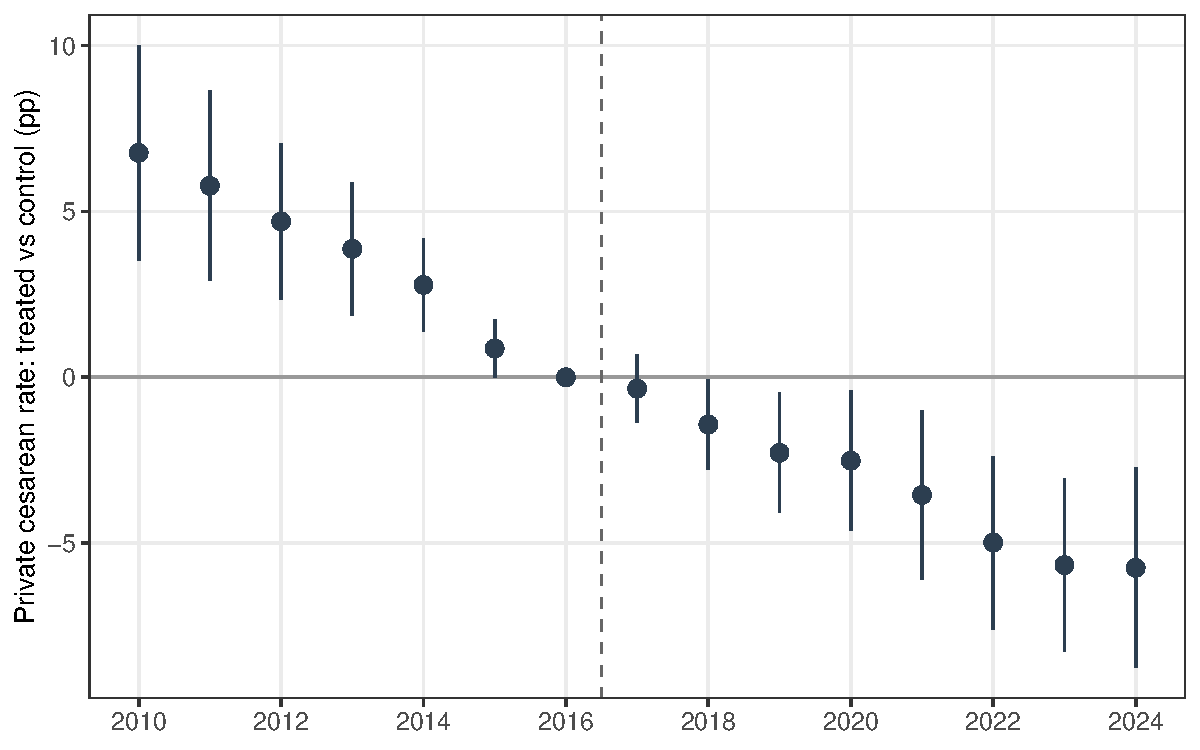
\includegraphics[width=0.8\textwidth]{../analysis/output/graphs/fig04_parto_adequado_es_sinasc.pdf}
\caption{Parto Adequado event study, treated versus control municipalities}\label{fig:pa_es}
\fignotes{For-profit cesarean rate, treated (participating for-profit hospital)
minus control municipalities, relative to 2016. The pre-existing downward trend
has no break at the 2017 onset (dashed line).}
\end{figure}


\begin{table}[H]
   \caption{\label{tab:parto_adequado} Parto Adequado DiD (does NOT survive the parallel-trends test)}
   \centering
\small\setlength{\tabcolsep}{5pt}
   \begin{tabular}{lcc}
      \toprule
      Dependent Variable: & \multicolumn{2}{c}{rate}\\
                                                        & Private (SINASC, annual) & Private (TISS, quarterly) \\   
      Model:                                            & (1)                      & (2)\\  
      \midrule
      \emph{Variables}\\
      Post (2017+) $\times$ Treated municipality $=$ 1  & -0.0659$^{***}$          & -0.0159\\   
                                                        & (0.0146)                 & (0.0136)\\   
\addlinespace[2pt]
      \midrule
      \emph{Fixed-effects}\\
      Municipality                                      & Yes                      & Yes\\  
      Year                                              & Yes                      & \\  
      Quarter                                           &                          & Yes\\  
      \midrule
      \emph{Fit statistics}\\
      Observations                                      & 7,660                    & 22,303\\  
      R$^2$                                             & 0.856                    & 0.776\\  
\bottomrule
   \end{tabular}
   
   \par \raggedright 
   \footnotesize\textit{Notes:} Treated = municipality with a participating \emph{Parto Adequado} Fase 2 private hospital (a diluted exposure; TISS has no hospital identifier). Weighted by private births (SINASC) / deliveries (TISS). SE clustered by municipality. \emph{The SINASC event study rejects parallel pre-trends} (2010--2015 joint test $F=4.5$, $p<0.001$): treated munis are on a pre-existing differential downward trend, so this DiD is not interpreted causally. \footnotesize Significance: *** p$<$0.01, ** p$<$0.05, * p$<$0.10.
\end{table}




\begin{table}[H]
   \caption{\label{tab:pretrend_robustness} \textbf{\emph{Parto Adequado}: covariate and treated-trend robustness}}
   \centering
\small\setlength{\tabcolsep}{5pt}\resizebox{\ifdim\width>\linewidth \linewidth\else\width\fi}{!}{%
   \begin{tabular}{lcccc}
      \toprule
      Dependent Variable: & \multicolumn{4}{c}{Cesarean rate}\\
                                   & Baseline        & + Covariates     & + Treated trend      & + Both \\
      Model:                       & (1)             & (2)              & (3)                  & (4)\\
      \midrule
      \emph{Variables}\\
      Treated $\times$ Post (2017+) & -0.0659$^{***}$ & -0.0508$^{***}$  & 0.0029               & 0.0042\\
                                   & (0.0146)        & (0.0145)         & (0.0099)             & (0.0099)\\   
\addlinespace[2pt]
      \midrule
      Municipality fixed effects & Yes             & Yes              & Yes                  & Yes\\  
      Year fixed effects & Yes             & Yes              & Yes                  & Yes\\  
      \midrule
      \emph{Fit statistics}\\
      Observations                 & 7,660           & 7,218            & 7,660                & 7,218\\  
\bottomrule
   \end{tabular}
}
   
   \par \raggedright 
   \footnotesize\textit{Notes:} SINASC for-profit cesarean rate, municipality-year 2010--2024, weighted by births. Column 1 is the baseline difference-in-differences; column 2 adds time-varying municipal covariates; column 3 adds a treated-cohort linear time trend; column 4 adds both. Covariates leave the differential pre-trend intact (joint 2010--2015 test still rejects, $p<0.01$); the treated linear trend absorbs the 2017 ``break'' entirely, confirming it is a pre-existing trend, not a treatment effect. Standard errors, clustered by municipality, are reported in parentheses. \footnotesize Significance levels: *** p$<$0.01, ** p$<$0.05, * p$<$0.10.
\end{table}




\begin{figure}[H]\centering
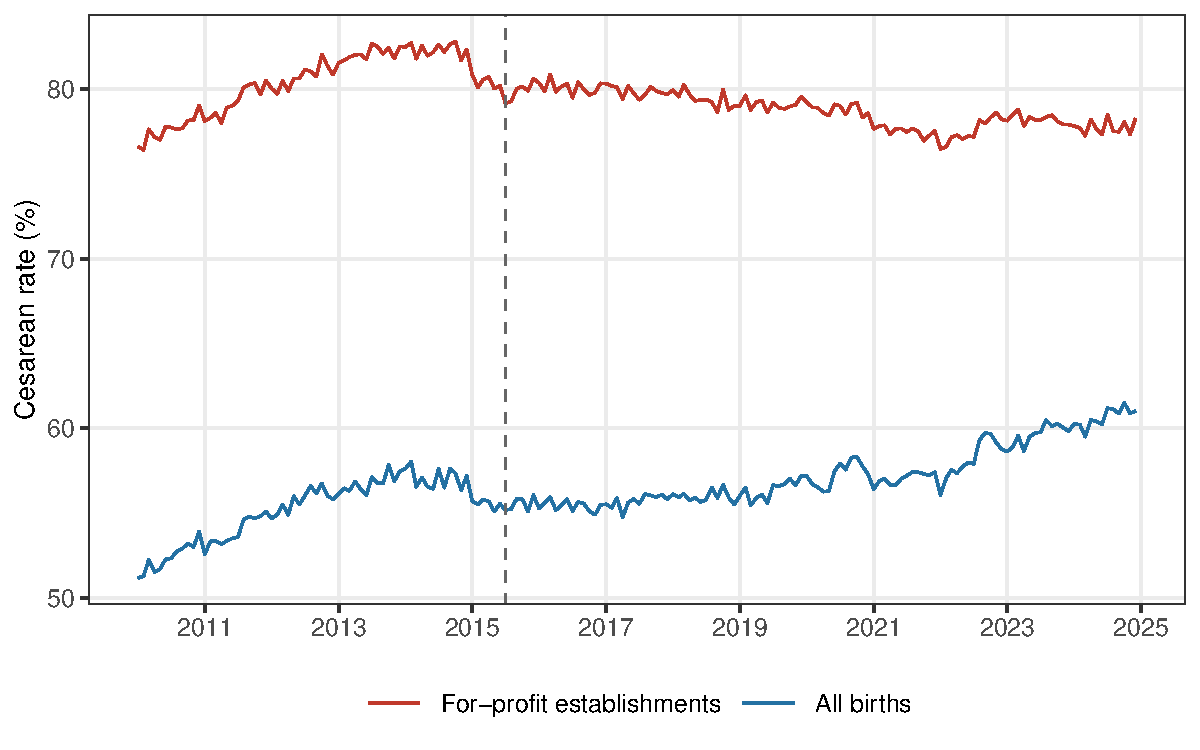
\includegraphics[width=0.8\textwidth]{../analysis/output/graphs/fig05_rn368_timeline.pdf}
\caption{National cesarean rate and the policy timeline}\label{fig:rn368}
\fignotes{Monthly cesarean rate, for-profit and all births.
Dashed line marks RN 368/2015.}
\end{figure}

\subsection{Additional robustness}

This subsection collects the supporting and robustness exhibits discussed in the
text. Table~\ref{tab:referee_robustness} re-estimates the weekend dip under a
time-varying sector classification, alternative rest-day definitions, and the
composition of weekend newborns. Table~\ref{tab:beneficiary_muni} replicates the
fee-gap null aggregating by the beneficiary's municipality, and
Table~\ref{tab:dip_region_period} shows that the dip survives a clinically clean
low-risk sample and is stable across regions and periods.
Table~\ref{tab:permutation} reports a descriptive ranking of the weekend dip
across all twenty-one two-day placebos, and Table~\ref{tab:no_indication} the
share of for-profit cesareans with no recorded clinical indication.
Table~\ref{tab:neonatal_suggestive} reports the suggestive, and statistically
weak, association between early-term shifting and neonatal admissions.


\begin{table}[H]
   \caption{\label{tab:referee_robustness} Referee-stage robustness: sector classification, rest-day definitions, newborn composition}
   \centering
\footnotesize\setlength{\tabcolsep}{3pt}
   \begin{tabular}{lccccc}
      \toprule
      Dependent Variables: & \multicolumn{3}{c}{Cesarean share} & \multicolumn{2}{c}{Outcome}\\
                                    & Cesarean, time-varying sector & Cesarean, Sunday only & Cesarean, rest days & Low Apgar      & Low birthweight \\   
      Model:                        & (1)                           & (2)                   & (3)                 & (4)            & (5)\\  
      \midrule
      \emph{Variables}\\
      Weekend                       & -0.0769$^{***}$               &                       &                     & 0.0019$^{***}$ & 0.0132$^{***}$\\   
                                    & (0.0046)                      &                       &                     & (0.0002)       & (0.0013)\\   
\addlinespace[2pt]
      Sunday                        &                               & -0.1081$^{***}$       &                     &                &   \\   
                                    &                               & (0.0071)              &                     &                &   \\   
\addlinespace[2pt]
      Rest day (weekend or holiday) &                               &                       & -0.0810$^{***}$     &                &   \\   
                                    &                               &                       & (0.0047)            &                &   \\   
\addlinespace[2pt]
      \midrule
      \emph{Fixed-effects}\\
      Municipality                  & Yes                           & Yes                   & Yes                 & Yes            & Yes\\  
      Year                          & Yes                           & Yes                   & Yes                 & Yes            & Yes\\  
      \midrule
      \emph{Fit statistics}\\
      Observations                  & 1,380,183                     & 1,455,272             & 1,455,272           & 1,447,875      & 1,455,272\\  
\bottomrule
   \end{tabular}
   
   \par \raggedright 
   \footnotesize\textit{Notes:} Private-sector municipality-date cells, SINASC 2010--2024, weighted by births. Column 1 reclassifies each birth's establishment with the natureza jur\'idica of its own year (2015--2024; earlier births use 2015). Columns 4--5 are composition checks: weekend (unscheduled) private births include fewer healthy scheduled term pregnancies, so newborn risk indicators shift mechanically. SE two-way clustered by municipality and date. \footnotesize Significance: *** p$<$0.01, ** p$<$0.05, * p$<$0.10.
\end{table}




\begin{table}[H]
   \caption{\label{tab:beneficiary_muni} Not a price story: beneficiary-municipality aggregation}
   \centering
\small\setlength{\tabcolsep}{5pt}\resizebox{\ifdim\width>\linewidth \linewidth\else\width\fi}{!}{%
   \begin{tabular}{lcc}
      \toprule
      Dependent Variable: & \multicolumn{2}{c}{Private cesarean rate}\\
      Model:                                        & (1)             & (2)\\
      \midrule
      \emph{Variables}\\
      Log economic fee gap (cesarean minus vaginal) & 0.0291          & -0.0131$^{**}$\\   
                                                    & (0.0176)        & (0.0062)\\   
\addlinespace[2pt]
      \midrule
      \emph{Fixed-effects}\\
      State                                         & Yes             & \\  
      Year                                          & Yes             & Yes\\  
      Municipality                                  &                 & Yes\\  
      \midrule
      \emph{Fit statistics}\\
      Observations                                  & 10,722          & 10,722\\  
      R$^2$                                         & 0.354           & 0.827\\  
\bottomrule
   \end{tabular}
}
   
   \par \raggedright 
   \footnotesize\textit{Notes:} TISS delivery events 2015--2024 aggregated by the beneficiary's municipality of residence (the baseline uses the provider municipality), weighted by deliveries; cells with at least 20 deliveries. The fee-gap null replicates. \footnotesize Significance: *** p$<$0.01, ** p$<$0.05, * p$<$0.10.
\end{table}




\begin{table}[H]
   \caption{\label{tab:dip_region_period} The private weekend dip: clean clinical sample, regions, and periods}
   \centering
\footnotesize\setlength{\tabcolsep}{2pt}
   \begin{tabular}{lccccccccc}
      \toprule
      Dependent Variable: & \multicolumn{9}{c}{Cesarean share}\\
                   & Clean low-risk  & North           & Northeast       & Southeast       & South           & Center-West     & 2010-2014       & 2015-2019       & 2020-2024 \\   
      Model:       & (1)             & (2)             & (3)             & (4)             & (5)             & (6)             & (7)             & (8)             & (9)\\  
      \midrule
      \emph{Variables}\\
      Weekend      & -0.0891$^{***}$ & -0.1072$^{***}$ & -0.0959$^{***}$ & -0.0671$^{***}$ & -0.0893$^{***}$ & -0.0780$^{***}$ & -0.0810$^{***}$ & -0.0776$^{***}$ & -0.0757$^{***}$\\   
                   & (0.0057)        & (0.0163)        & (0.0089)        & (0.0054)        & (0.0084)        & (0.0095)        & (0.0061)        & (0.0048)        & (0.0041)\\   
\addlinespace[2pt]
      \midrule
      \emph{Fixed-effects}\\
      Municipality & Yes             & Yes             & Yes             & Yes             & Yes             & Yes             & Yes             & Yes             & Yes\\  
      Year         & Yes             & Yes             & Yes             & Yes             & Yes             & Yes             & Yes             & Yes             & Yes\\  
      \midrule
      \emph{Fit statistics}\\
      Observations & 952,302         & 153,312         & 298,836         & 508,597         & 267,885         & 226,642         & 528,502         & 489,898         & 436,872\\  
\bottomrule
   \end{tabular}
   
   \par \raggedright 
   \footnotesize\textit{Notes:} Private-sector municipality-date cells, weighted by births. \emph{Clean low-risk} keeps births with no recorded schedulable indication: cephalic presentation, singleton, term (37--41 weeks), no prior cesarean (multiparity allowed, unlike Robson 1--2). SE two-way clustered by municipality and date. \footnotesize Significance: *** p$<$0.01, ** p$<$0.05, * p$<$0.10.
\end{table}



\begin{table}[H]\centering
\caption{\textbf{Descriptive ranking: the weekend dip across all 21 two-day placebos}}
\label{tab:permutation}\small
\small\setlength{\tabcolsep}{4pt}\resizebox{\ifdim\width>\linewidth \linewidth\else\width\fi}{!}{%
\begin{tabular}{lc}
\toprule
Pseudo rest-day pair & Private cesarean dip (pp) \\
\midrule
Sun+Sat (true weekend) & -8.11 \\
Sun+Fri & -3.90 \\
Sun+Thu & -3.62 \\
Sun+Wed & -3.20 \\
Sun+Tue & -3.16 \\
Sun+Mon & -1.78 \\
Fri+Sat & -1.58 \\
Thu+Sat & -1.36 \\
Wed+Sat & -0.98 \\
Tue+Sat & -0.95 \\
Mon+Sat & 0.26 \\
Thu+Fri & 1.37 \\
Wed+Fri & 1.70 \\
Tue+Fri & 1.72 \\
Wed+Thu & 1.87 \\
Tue+Thu & 1.90 \\
Tue+Wed & 2.21 \\
Mon+Fri & 2.77 \\
Mon+Thu & 2.93 \\
Mon+Wed & 3.24 \\
Mon+Tue & 3.27 \\
\bottomrule
\end{tabular}
}
\\[2pt]\footnotesize\textit{Notes:} Each row re-estimates the private-sector weekend term of Equation~\eqref{eq:scheduling}, treating a different pair of weekdays as the ``rest days'' (SINASC 2010--2024, municipality-date cells, municipality and year fixed effects, weighted by births). The true weekend (Sun+Sat) is the most negative of all 21 placebos (rank 1 of 21). Because the days of the week are not exchangeable under a known assignment mechanism, this is a descriptive ranking, not an exact randomization-inference $p$-value.
\end{table}

\begin{table}[H]\centering
\caption{\textbf{Private cesareans with no recorded clinical indication}}
\label{tab:no_indication}\small
\small\setlength{\tabcolsep}{4pt}\resizebox{\ifdim\width>\linewidth \linewidth\else\width\fi}{!}{%
\begin{tabular}{cc}
\toprule
Year & Share with no indication ICD-10 code (\%) \\
\midrule
2015 & 87.2 \\
2016 & 88.2 \\
2017 & 87.9 \\
2018 & 88.1 \\
2019 & 87.9 \\
2020 & 89.0 \\
2021 & 89.2 \\
2022 & 90.0 \\
2023 & 90.8 \\
2024 & 91.2 \\
\bottomrule
\end{tabular}
}
\\[2pt]\footnotesize\textit{Notes:} TISS private cesarean deliveries, 2015--2024. A delivery is coded ``no indication'' when the primary diagnosis (ICD-10 code) is a delivery-outcome code (O80--O84) or blank, rather than an ICD-10 code recording a recognized cesarean indication (malpresentation, disproportion, placental or fetal complications, obstructed labor, etc.). Diagnosis coding in claims is incomplete, so this describes recorded indications, not clinical necessity.
\end{table}


\begin{table}[H]
   \caption{\label{tab:neonatal_suggestive} \textbf{Early-term shifting and neonatal hospital use}}
   \centering
\small\setlength{\tabcolsep}{5pt}\resizebox{\ifdim\width>\linewidth \linewidth\else\width\fi}{!}{%
   \begin{tabular}{lccc}
      \toprule
 & (1)      & (2)      & (3)\\  
\addlinespace[2pt]
 & \multicolumn{2}{c}{Perinatal-condition admissions per private birth} & All infant admissions per private birth\\
      \midrule
      Share of private births at 37--38 weeks & 0.0044   &          & -0.0084\\   
                                              & (0.0097) &          & (0.0540)\\   
\addlinespace[2pt]
      For-profit cesarean rate                &          & 0.0094   &   \\   
                                              &          & (0.0070) &   \\   
\addlinespace[2pt]
      \midrule
      Municipality fixed effects & Yes      & Yes      & Yes\\  
      Year fixed effects & Yes      & Yes      & Yes\\  
      \midrule
      Observations                            & 4,284    & 4,284    & 4,284\\  
\bottomrule
   \end{tabular}
}
\begin{minipage}{\linewidth}\footnotesize
\textit{Notes:} Municipality-year cells, 2015--2024, weighted by private births; cells with at least 50 private births. Infant admissions are TISS hospital events of beneficiaries in the $<$1 age band, at the provider municipality; perinatal conditions are primary diagnoses of conditions originating in the perinatal period. Ecological and correlational, a corroboration of the early-term margin, not a causal estimate. Standard errors, clustered by municipality, are reported in parentheses. \footnotesize Significance levels: *** p$<$0.01, ** p$<$0.05, * p$<$0.10.
\end{minipage}
\end{table}




% =============================================================================
\section{Supplementary robustness and inference}\label{app:referee}
% =============================================================================
This appendix reports supplementary validation of the timing indicator, few-cluster
inference for the fee channel, and sample-construction accounting.
Table~\ref{tab:robson_validation} verifies that the cesarean-timing indicator is
internally consistent across Robson groups: group 1 (spontaneous labor) carries no
prelabor cesareans, so its weekend dip is entirely in-labor and cannot come from
prelabor scheduling, and a formal test cannot distinguish the group-1 dip from the
group-10 (preterm) dip. Table~\ref{tab:feegap_ci} reports the fee-gap coefficient
with confidence intervals against a pre-specified economic-equivalence region,
showing the estimate is sign-unstable rather than a precise zero.
Table~\ref{tab:fee_base_econ} shows the fee-gap null is unchanged when the vaginal
fee is measured by the base delivery fee alone, so it does not depend on the
endogenous billed labor-assistance hours. Table~\ref{tab:fewcluster} re-does
inference on the fee-shock coefficient with a wild-cluster bootstrap over the small
number of state clusters. Table~\ref{tab:sampleflow} documents sample construction,
and Table~\ref{tab:timing_missing} shows that missingness of the cesarean-timing
indicator is balanced across weekdays and weekends, so the prelabor/in-labor split
is not a missingness artifact.

\begin{table}[H]\centering
\caption{\textbf{Internal consistency of the cesarean-timing indicator across Robson groups}}
\label{tab:robson_validation}
\small
\small\setlength{\tabcolsep}{4pt}\resizebox{\ifdim\width>\linewidth \linewidth\else\width\fi}{!}{%
\begin{tabular}{lrr}
\toprule
Robson group & Cesareans & Share coded prelabor (\%) \\
\midrule
01 & 1,499,945 & 0.0 \\
02 & 2,211,444 & 84.7 \\
03 &   694,312 & 0.0 \\
04 &   922,035 & 85.0 \\
05 & 3,780,923 & 56.5 \\
06 &   261,292 & 53.0 \\
07 &   340,458 & 52.0 \\
08 &   376,493 & 56.7 \\
09 &    45,713 & 49.8 \\
10 & 1,058,662 & 53.8 \\
\midrule
\multicolumn{3}{p{0.9\linewidth}}{\footnotesize Group 1 (spontaneous labor) has a 0.0\% prelabor share, as it must; its for-profit weekend dip of -6.5 pp is therefore entirely in-labor (in-labor component -5.5 pp). A formal test cannot distinguish the group-1 dip from the group-10 (preterm) dip ($p=0.18$), so the preterm placebo is weak.} \\
\bottomrule
\end{tabular}
}
\\[2pt]\footnotesize\textit{Notes:} SINASC 2010--2024, cesareans with a valid before/during-labor code. Robson 1 = nulliparous, term, singleton, cephalic, spontaneous labor; Robson 2 = same but induced or prelabor cesarean.
\end{table}

\begin{sidewaystable}\centering
\caption{\textbf{The fee-gap coefficient against two yardsticks: an equivalence region and the canonical price response}}
\label{tab:feegap_ci}
\small
\small\setlength{\tabcolsep}{4pt}\resizebox{\ifdim\width>\linewidth \linewidth\else\width\fi}{!}{%
\begin{tabular}{lcccccc}
\toprule
Specification & Coefficient & 95\% CI & Clusters & In $[-0.02,0.02]$? & Excludes Grant? & Excludes GKM?
\\
\midrule
State fixed effects & +0.0469 & [-0.0020, +0.0958] &  27 & not within & not excluded & not excluded \\
Municipality fixed effects & -0.0163 & [-0.0340, +0.0015] & 719 & not within & excluded & excluded \\
State fixed effects + controls & +0.0166 & [-0.0306, +0.0638] &  27 & not within & not excluded & not excluded \\
Municipality fixed effects + controls & -0.0143 & [-0.0321, +0.0036] & 714 & not within & excluded & excluded \\
\bottomrule
\end{tabular}
}
\begin{minipage}{\linewidth}\footnotesize
\textit{Notes:} Coefficient on the log economic fee gap from Table~\ref{tab:fees}. The equivalence region $[-0.02, 0.02]$ corresponds to a 2 percentage-point change in the cesarean share per log point of the fee gap. The final two columns ask whether the interval excludes the price response the literature has estimated. \citet{gruber1999physician} report about four percentage points of cesarean rate per US\$1{,}000 of the cesarean-vaginal fee differential; re-estimating that response on corrected data, \citet{grant2009} obtains about one point, which he describes as a quarter of the original. At our delivery-weighted mean cesarean fee of R\$1,941 the two are 0.72 and 2.87 percentage points per log point of the fee gap; the conversion uses US consumer prices between 1990 and 2020 and the World Bank purchasing-power factor for Brazil, and is deliberately rough. Two things follow, and the paper states both. No interval fits inside the equivalence region, so these data do not establish that the price response is negligible. And the two fixed-effect schemes disagree about both magnitudes: the within-municipality intervals exclude them, the state-level intervals, estimated on twenty-seven clusters, are too wide to. The sign itself is unstable across the two schemes. The economic argument of Section~\ref{sec:notprice} does not rest on this table: the 0.10 to 0.35 log point negative fee gap of the largest states would move the cesarean rate by about a quarter of a percentage point at Grant's magnitude and about one point at the original, against a for-profit--public gap of 35 points.
\end{minipage}
\end{sidewaystable}


\begin{table}[H]
   \caption{\label{tab:fee_base_econ} \textbf{The fee-gap null does not depend on the endogenous labor-assistance hours}}
   \centering
\small\setlength{\tabcolsep}{4pt}\resizebox{\ifdim\width>\linewidth \linewidth\else\width\fi}{!}{%
   \begin{tabular}{lcccc}
      \toprule
      Dependent Variable: & \multicolumn{4}{c}{Private-insurance cesarean rate}\\
                                         & Base vaginal fee & Base vaginal fee & Economic vaginal fee & Economic vaginal fee \\
      Model:                             & (1)            & (2)            & (3)                & (4)\\  
      \midrule
      \emph{Variables}\\
      Log fee gap (base vaginal fee)     & 0.0358$^{*}$   & -0.0192$^{**}$ &                    &   \\   
                                         & (0.0196)       & (0.0092)       &                    &   \\   
\addlinespace[2pt]
      Log fee gap (economic vaginal fee) &                &                & 0.0473$^{*}$       & -0.0163$^{*}$\\   
                                         &                &                & (0.0241)           & (0.0090)\\   
\addlinespace[2pt]
      \midrule
      \emph{Fixed-effects}\\
      State                              & Yes            &                & Yes                & \\  
      Year                               & Yes            & Yes            & Yes                & Yes\\  
      Municipality                       &                & Yes            &                    & Yes\\  
      \midrule
      \emph{Fit statistics}\\
      Observations                       & 5,176          & 5,176          & 5,176              & 5,176\\  
      R$^2$                              & 0.315          & 0.849          & 0.334              & 0.849\\  
\bottomrule
   \end{tabular}
}
   
   \par \raggedright 
   \footnotesize\textit{Notes:} Municipality-year cells built from event-level TISS claims, weighted by deliveries. The base fee gap uses only the delivery procedure fee; the economic fee gap adds the separately-billed hourly labor-assistance fee to the vaginal fee. The coefficient is small and sign-unstable under both definitions, so the null is not an artifact of the endogenous billed hours. SE clustered by the fixed-effect geography. \footnotesize Significance levels: *** p$<$0.01, ** p$<$0.05, * p$<$0.10.
\end{table}



\begin{table}[H]\centering
\caption{Few-cluster inference for the fee channel}
\label{tab:fewcluster}
\small
\small\setlength{\tabcolsep}{4pt}\resizebox{\ifdim\width>\linewidth \linewidth\else\width\fi}{!}{%
\begin{tabular}{lc}
\toprule
Quantity & Value \\
\midrule
Fee-shock coefficient ($\Delta$ cesarean on $\Delta$ fee gap) & -0.0127 \\
Number of state clusters & 22 \\
Cluster-robust analytic $p$-value & 0.275 \\
Wild-cluster (Webb) bootstrap $p$-value & 0.210 \\
\bottomrule
\end{tabular}
}
\\[2pt]\footnotesize\textit{Notes:} State-year first differences, weighted by deliveries, 9,999 Webb-weight wild-cluster bootstrap draws with the state as the cluster. The fee-shock coefficient is not distinguishable from zero under proper few-cluster inference. The municipality fixed-effect specifications in Table~\ref{tab:not_a_price} have several hundred clusters and are unaffected.
\end{table}

\begin{table}[H]\centering
\caption{Sample construction, SINASC birth records}
\label{tab:sampleflow}
\small
\small\setlength{\tabcolsep}{4pt}\resizebox{\ifdim\width>\linewidth \linewidth\else\width\fi}{!}{%
\begin{tabular}{lr}
\toprule
Step & Records \\
\midrule
Raw SINASC birth records & 42,003,663 \\
Restrict to 2010--2024 & 42,003,663 \\
Private (for-profit) or public establishment & 27,171,480 \\
\quad of which: valid Robson group (2014+) & 22,930,574 \\
\quad of which: valid before/during-labor code (cesareans) & 24,624,121 \\
\bottomrule
\end{tabular}
}
\\[2pt]\footnotesize\textit{Notes:} The Robson classification is populated from 2014; the before/during-labor timing code is well populated from about 2012. Analyses that need each variable use the corresponding sub-sample, as noted in each table.
\end{table}

\begin{table}[H]\centering
\caption{\textbf{Missingness of the cesarean-timing indicator is balanced across the week}}
\label{tab:timing_missing}
\small
\small\setlength{\tabcolsep}{4pt}\resizebox{\ifdim\width>\linewidth \linewidth\else\width\fi}{!}{%
\begin{tabular}{lcc}
\toprule
Sector & Weekday (\%) & Weekend (\%) \\
\midrule
For-profit & 16.04 & 16.09 \\
Public & 18.12 & 17.81 \\
\bottomrule
\end{tabular}
}
\\[2pt]\footnotesize\textit{Notes:} Share of cesareans with a missing before/during-labor code, SINASC 2010--2024. The near-identical weekday and weekend rates imply the prelabor/in-labor split is not driven by differential missingness across the week.
\end{table}


\subsection{Multiple hypothesis testing}\label{app:multiple}

The paper reports more than one test in two places where a reader may worry about
selective reporting: the heterogeneity of the weekend dip, and the differences
between for-profit and public establishments in gestational and newborn outcomes.
We therefore group the hypotheses into three pre-specified families and adjust
within each. Family A is the for-profit calendar gradient of
Table~\ref{tab:pooled_did}, which tests the weekend, holiday, and eve interactions
together. Family B is the heterogeneity of the weekend dip, comprising the
obstetrician-density and maternal-education interactions of
Table~\ref{tab:heterogeneity} and the cooperative-insurer contrast of
Table~\ref{tab:modality}. Family C is the set of for-profit-versus-public outcome
differences of Table~\ref{tab:health}: early-term birth, low birthweight, and low
Apgar score. Families are defined by the substantive question a reader would pose,
not by the outcome of the test. Table~\ref{tab:multiple_testing} reports, within
each family, the Holm-Bonferroni adjusted $p$-value \citep{holm1979}, which controls
the familywise error rate, and the Benjamini-Hochberg $q$-value
\citep{benjamini1995}, which controls the false discovery rate. The adjustments do
not change any conclusion: the estimates that are
individually significant remain so, and the cooperative-insurer contrast, which was
insignificant to begin with, stays insignificant. The precision comes from sample
sizes in the millions rather than from a fortunate choice among tests.

\begin{table}[H]
   \caption{\label{tab:multiple_testing} Multiple-hypothesis adjustment within pre-specified families}
   \centering
\small\setlength{\tabcolsep}{5pt}\resizebox{\ifdim\width>\linewidth \linewidth\else\width\fi}{!}{%
   \begin{tabular}{lcccc}
      \toprule
      Hypothesis & Estimate & Unadjusted $p$ & Holm $p$ & BH $q$ \\
      \midrule
      \emph{A. For-profit calendar gradient} & & & & \\
      \quad For-profit $\times$ Weekend & -0.0182 & 0.006 & 0.006 & 0.006 \\
      \quad For-profit $\times$ National holiday & -0.0244 & $<$0.001 & $<$0.001 & $<$0.001 \\
      \quad For-profit $\times$ Eve of rest day & -0.0095 & 0.002 & 0.004 & 0.003 \\
      \addlinespace[3pt]
      \emph{B. Heterogeneity in the weekend dip} & & & & \\
      \quad Weekend $\times$ Low obstetrician density & -0.0223 & 0.005 & 0.010 & 0.008 \\
      \quad Weekend $\times$ Mother has 8+ years of schooling & 0.1441 & $<$0.001 & $<$0.001 & $<$0.001 \\
      \quad Physician-owned cooperative insurer & 0.0084 & 0.350 & 0.350 & 0.350 \\
      \addlinespace[3pt]
      \emph{C. For-profit--public outcome differences} & & & & \\
      \quad Early-term birth (37--38 weeks) & 0.1087 & $<$0.001 & $<$0.001 & $<$0.001 \\
      \quad Low birthweight ($<$2500g) & -0.0290 & $<$0.001 & $<$0.001 & $<$0.001 \\
      \quad Five-minute Apgar $<$ 7 & -0.0055 & $<$0.001 & $<$0.001 & $<$0.001 \\
      \addlinespace[3pt]
\bottomrule
   \end{tabular}
}
   
   \par \raggedright 
   \footnotesize\textit{Notes:} Each family collects the hypotheses that the paper tests jointly. Family A is the within-municipality-day for-profit calendar gradient of Table~\ref{tab:pooled_did}; family B the heterogeneity tests of Tables~\ref{tab:heterogeneity} and~\ref{tab:modality}; family C the for-profit--public outcome differences of Table~\ref{tab:health}. Holm $p$ is the Holm--Bonferroni adjusted $p$-value \citep{holm1979}, which controls the familywise error rate within the family; BH $q$ is the Benjamini--Hochberg false-discovery-rate $q$-value \citep{benjamini1995}. Estimates and unadjusted $p$-values reproduce the corresponding columns of the source tables.
\end{table}




% The supplement now carries citations of its own (the multiple-testing
% procedures), so it needs its own reference list. Compile with:
%   pdflatex supplement ; bibtex supplement ; pdflatex supplement (x2)
\bibliographystyle{plainnat-rev}
\bibliography{refs}

\end{document}
